
\setcounter{mtc}{2} %indique le numéro réel du chapitre, pour la mini table des matières
\chapter{Mise en situation}
\minitoc  %insert la minitoc

\graphicspath{{Chapitre1/figures/}}
%==============================================================================
\pagestyle{fancy}
\fancyhf{}
\fancyhead[R]{\bfseries\rightmark}
\fancyfoot[R]{\thepage}
\renewcommand{\headrulewidth}{0.5pt}
\renewcommand{\footrulewidth}{0pt}
\renewcommand{\chaptermark}[1]{\markboth{\MakeUppercase{\chaptername~\thechapter. #1 }}{}}
\renewcommand{\sectionmark}[1]{\markright{\thechapter.\thesection~ #1}}

\begin{spacing}{1.5}

%==============================================================================
\section*{Introduction}
Avant de commencer à détailler le travail réalisé, il est indispensable d'introduire l'organisme d'accueil afin de se faire une idée sur son domaine d'activité, la situation actuelle qui l'a motivé à entreprendre notre projet, ainsi que son orientation.\\
Une fois entamée, nous enchaînerons avec la présentation de la problématique, suivie d'une description sommaire du sujet du projet et des concepts clés associés.\\
La méthodologie employée tout au long de sa mise en œuvre sera traitée vers la fin du chapitre.


%==============================================================================
\section{Présentation de l'organisme d'accueil}
%-----------------------------------------------------------------------------------
\subsection{L'entreprise "IT SERV"}
IT SERV est une société de services et de conseil exerçant dans le domaine des Technologies de l'Information et de la Communication.
Fondée en 2008, elle a très tôt opté pour un positionnement stratégique sur les activités de conseil et de services dans le secteur des TIC en Tunisie. Elle a pour but de fournir des services à forte valeur ajoutée à ses clients. Dans ce cadre, elle vise essentiellement à les orienter vers l'adoption des technologies modernes, à maximiser l'efficacité et l'efficience de leur organisation et à optimiser leurs processus.\\
Ses valeurs fondamentales s'articulent autour de la satisfaction des clients d'une part et l'épanouissement et l'évolution de ses ingénieurs et consultants d'autre part. La figure \ref{fig:organigramme} présente la hiérarchie générale de l'entreprise.\\

\begin{figure}[h]
\centering
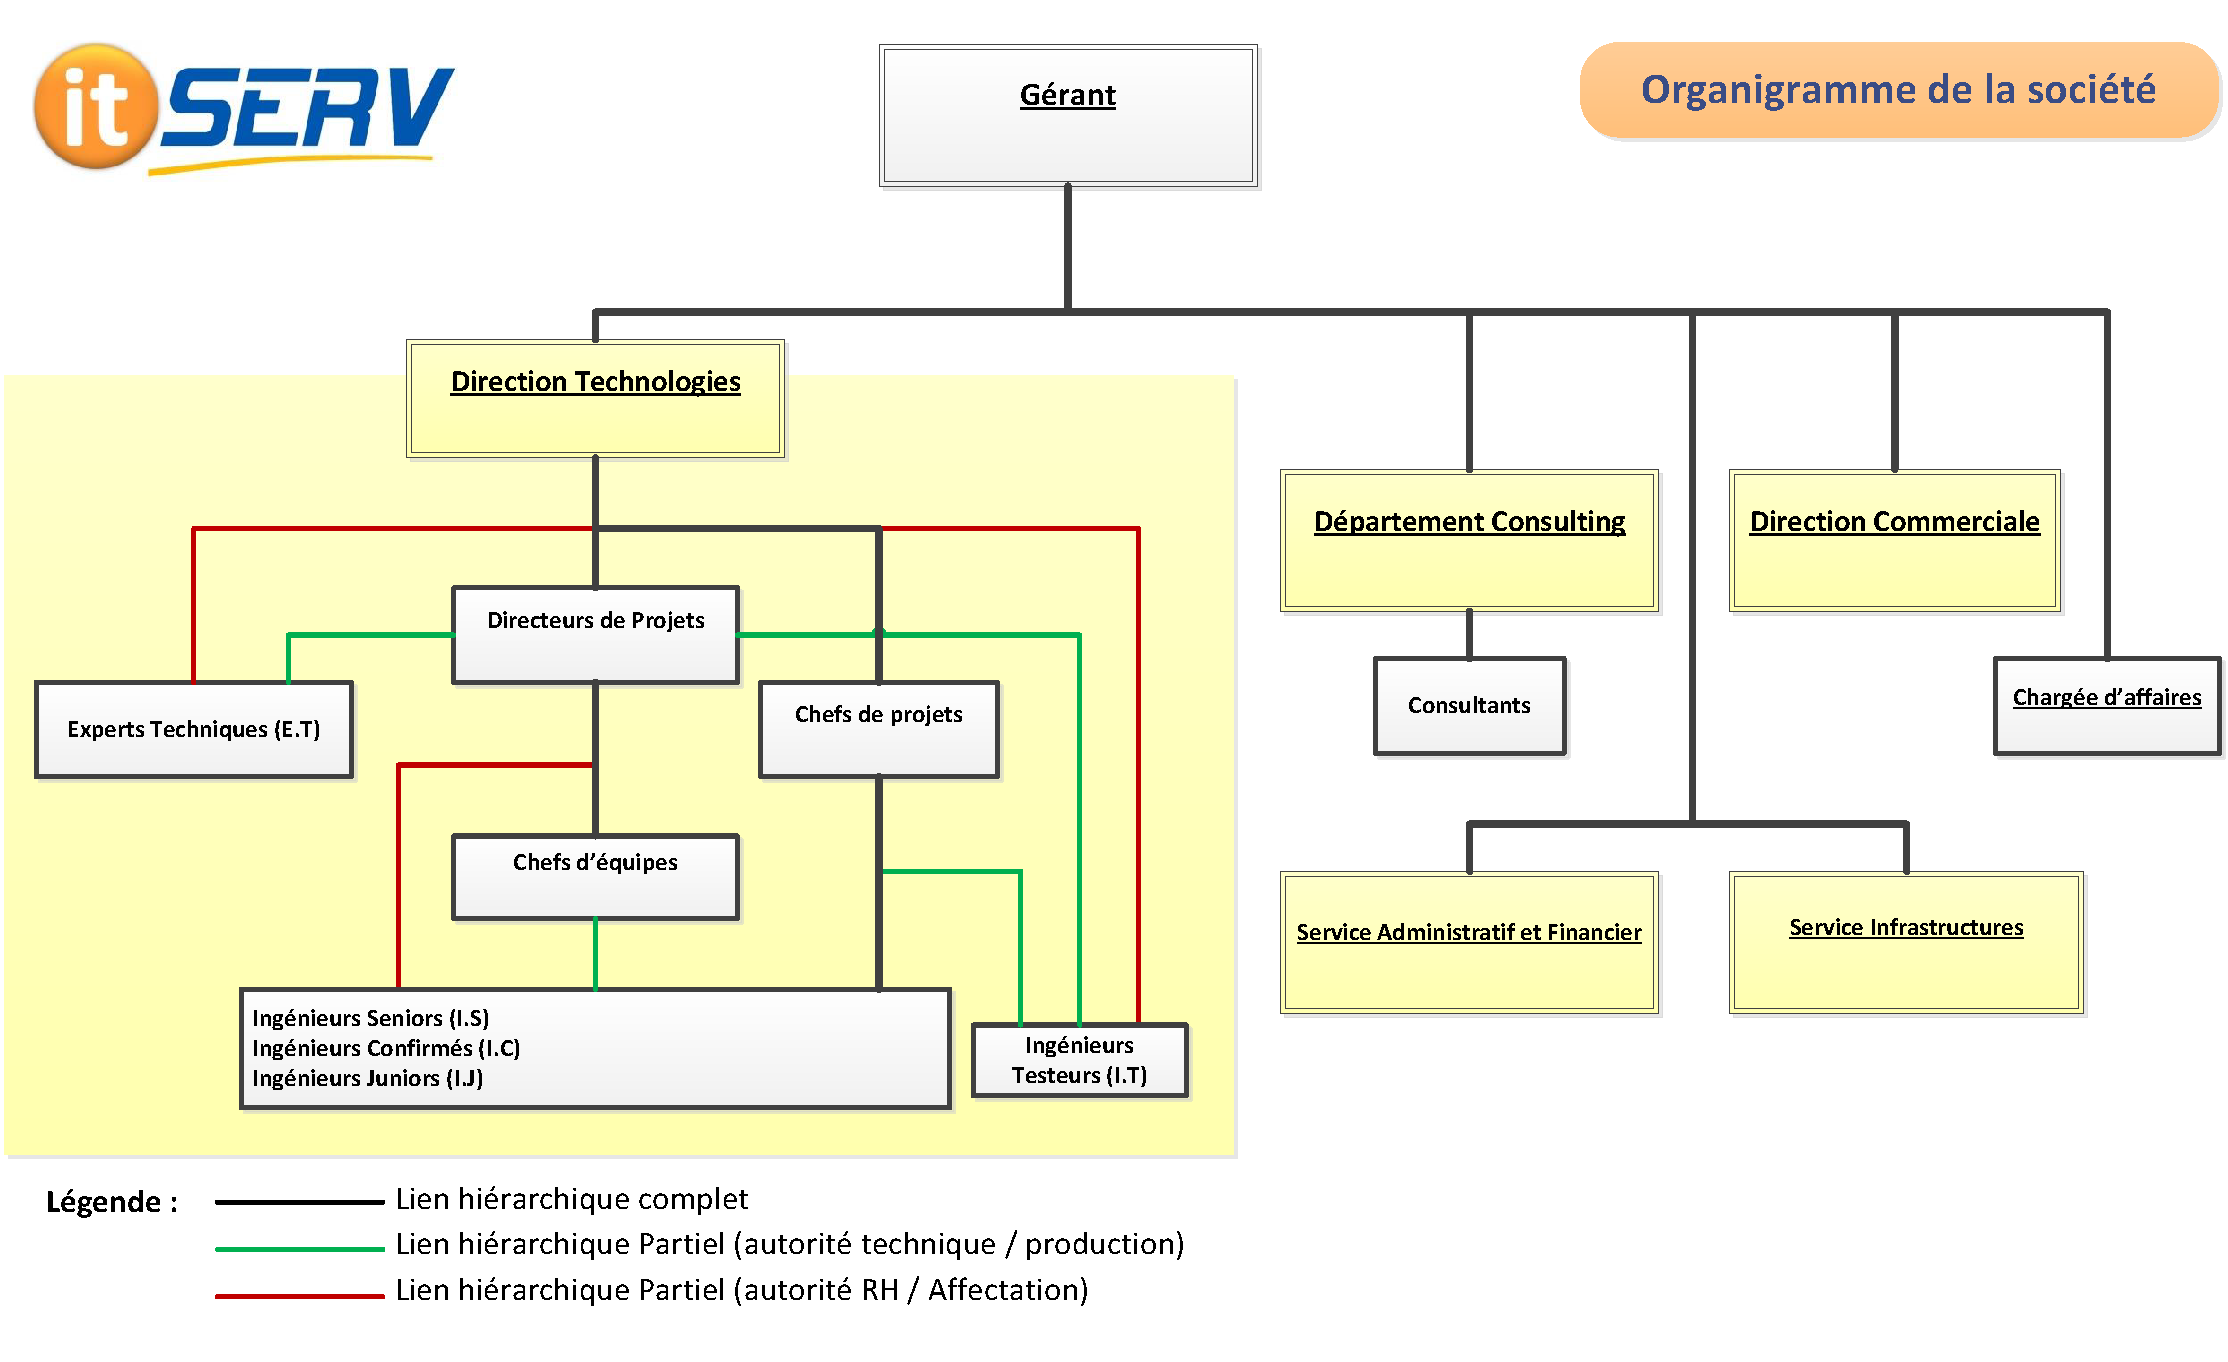
\includegraphics[scale=0.8]{organigramme.png}
\caption{Organigramme de l'entreprise}
\label{fig:organigramme}
\end{figure}

En plein essor, l'entreprise jouit d'une forte croissance sur tous les plans : chiffre d'affaires, résultats, effectifs, périmètre de compétence, portefeuille clients, etc. Cette réussite, à la fois en local et à l'international, constitue un facteur de stabilité et un facteur de confiance en soi pour ses clients et ses collaborateurs. Les graphiques de la figure \ref{statistiquesCroissance} fournissent plus de détail sur l'état actuel des lieux.\\

\begin{figure}[h]
\centering
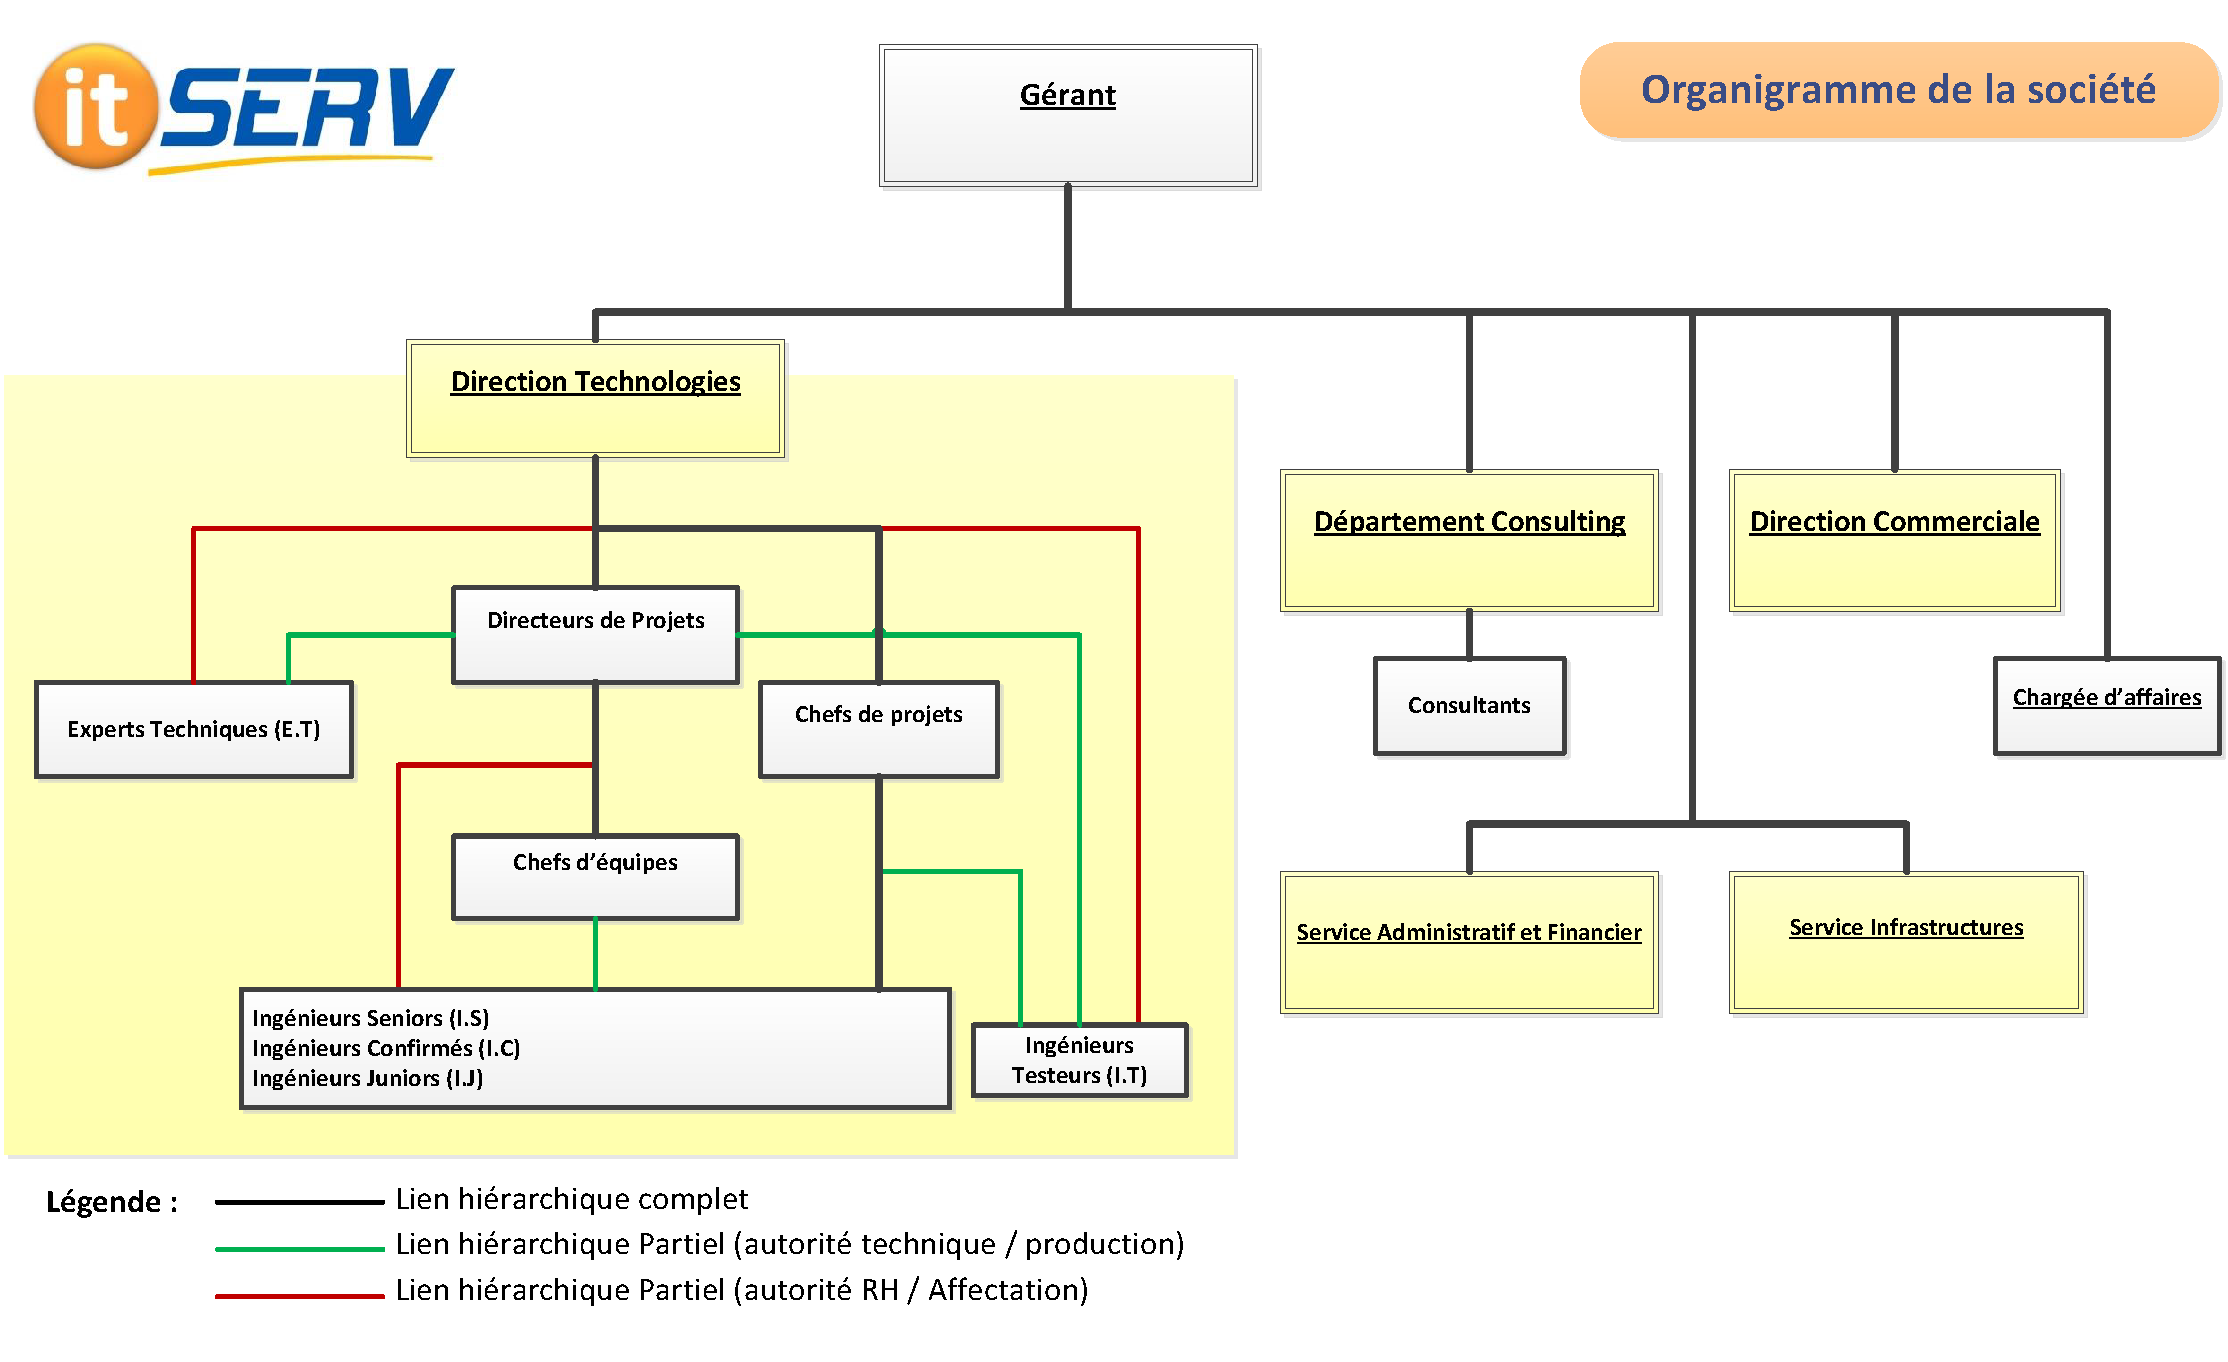
\includegraphics[scale=0.8]{organigramme.png}
\caption{Chiffre d'affaires, Croissance en nombres, Statistiques...}
\label{statistiquesCroissance}
\end{figure}

IT SERV favorise les partenariats s'inscrivant dans la continuité et la durée. En effet elle établit avec la majorité de ses clients des accords cadre, leur permettant de profiter de prix étudiés et de conditions avantageuses en matière de disponibilité, de priorité et d'engagement au plus haut niveau. Cette démarche stratégique lui permet d'avoir en contrepartie une visibilité long terme sur les commandes et les projets de ses clients, de dimensionner ses équipes en conséquence et d'optimiser son investissement en formation et mise à niveau de ses cadres en recherche \& développement.

%-----------------------------------------------------------------------------------
\subsection{Domaine d'expertise}
Les prestations d'IT SERV s'articulent autour de quatre offres :
\begin{itemize}
\item Consulting IT
    \item Intégration \& Développement
    \item Expertise Télécoms
    \item Nearshore Outsourcing
\end{itemize}
L'entreprise vise la réalisation de missions complexes ayant un apport conséquent pour ses clients, dans un cadre de partenariat bénéfique pour les deux parties. La réussite de toutes ses missions et l'atteinte des objectifs ont instauré des relations de confiance très durables et un élargissement progressif du périmètre d'intervention.

\begin{figure}[!ht]
\centering
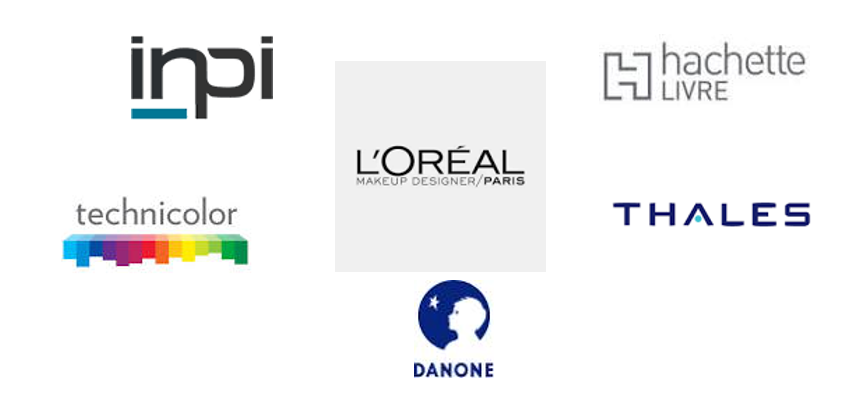
\includegraphics[scale=0.8]{reference.png}
\caption{Références de l'entreprise}
\label{refenrences}
\end{figure}

Plus récemment, l'entreprise aspire à élargir son éventail d'offres et entrevoit de se convertir en un éditeur de logiciel à part entière.


%==============================================================================
\section{Problématiques et motivations}
De nos jours, la gestion de projet s'impose dans les structures de toutes tailles comme le mode d'organisation par excellence.\\
Un projet désigne un ensemble finalisé d'activités et d'actions entreprises dans le but de répondre à un besoin, soumis à des contraintes bien définies, généralement dans des délais fixés avec une allocation budgétaire plafonnée. La gestion de projet quant à elle, représente la démarche visant à organiser de bout en bout le bon déroulement d'un projet.\\
Celle-ci revient généralement à la gestion de multiples facettes, notamment :
\begin{itemize}
\item La planification
    \item La gestion budgétaire
    \item Le pilotage des risques
    \item La gestion du changement
    \item La gestion des interventions
    \item La gestion des mises à jour
    \item La gestion des ressources
\end{itemize}
\

Avec les projets de plus en plus complexes auxquels les entreprises font face, gérer tous les flux d'information en perpétuel changement d'un projet se révèle être une tâche des plus ardues pour les chefs de projets. Sans un système efficace de traitement des données et d'achemeninement de l'information, ceux-ci finissent par être submergés par les requêtes, et se retrouvent le plus souvent dépassés par les événements. Ceci se reflète en conséquence par un manquement au niveau de la réponse aux attentes de l'une ou plusieurs des parties prenantes au projet, qui, souvent dû à des contraintes de disponibilité, restent trop longtemps en déphasage avec les dernières fluctuations et les mises à jour du projet.\\
C'est là que réside le cœur de la problématique : réussir à synchroniser de manière efficace toutes les parties prenantes à un projet avec l'état actuel de ce dernier, en distinguant le chef de projet en tant que pièce maîtresse de sa supervision.\\
\\
Le projet présent a pour but de répondre à ce problème en fournissant une solution logicielle dédiée à la gestion de projets. La solution se doit de répondre adéquatement aux attentes des chefs de projets en termes de fonctionnalités, mais aussi fournir un point pivotal d'aide à la décision pour les dirigeants de l'entreprise. En effet, les données récupérées tout au long de son exercice devront être en mesure d'être synthétisées en des données actionables, capables d'orienter les dirigeants de l'entreprise dans leur prise de décisions stratégiques quant à la détermination des clients les plus profitables, les partenariats les plus importants, etc.\\
Au sein de l'environnement extrêmement concurrentiel dans lequel exerce l'entreprise, et au vu du poids dont relève sa prestation de consulting en termes de gestion de bout en bout de projets, il est clair qu'une solution dédidée à la gestion du portefeuille de projets de l'entreprise avec ses clients constituerais un point fort face à la concurrence et impacterais positivement l'image de la société en influençant grandement le niveau de satisfaction de ses clients.\\
\\
Outre l'apport de l'application pour la gestion de ses propres projets en interne, dans l'optique de sa conversion en un éditeur de logiciel, IT SERV entrevoit de développer une offre autour d'une version SaaS de l'application.\\
 Dans ce cadre, le développement d'une interface de gestion et de monitoring de l'aspect SaaS de l'application s'impose en tant que partie à part entière du projet. Elle se verras traîtée plus en détail au cours du chapitre \ref{chapterX}.


%==============================================================================
\section{Méthodologie de travail}
Pour la réalisation d'un projet informatique d'envergure, il est indispensable de suivre une méthodologie de travail bien établie, prenant en compte les spécificités du projet, dans le but de garantir un niveau optimal de rendement tout au long de sa réalisation.
%-----------------------------------------------------------------------------------
\subsection{Choix méthodologique}
Les avancées majeures dans l'univers de l'informatque ont été accompagnées d'une révolution dans la manière de faire et de penser pour produire des logiciels. Celle-ci a éventuellement donnée naissance au processus unifié et au mouvement de déveoppement agile, qui se caractérisent par le développement de manière itérative et incrémentale.\\
Les deux méthodologies initialement considérées pour la mise en œuvre du projet ont été RUP \cite{RUP} et SCRUM \cite{SCRUM}, chacune mettant en avant les principaux avantages du processus unifié et des méthodes agiles, respectivement.\\
\\
À première vue, le processus unifié semble assez similaire aux méthodes agiles. Néanmoins, il s'en distingue par certaines caractéristiques :
\begin{itemize}
\item Piloté par les cas d'utilisation et les riques
    \item Centré sur l'architecture
    \item Prescrit un niveau élévé de formalisme
    \item Préconise un travail considérable sur les spécifications en amont
\end{itemize}
Plus particulièrement, RUP s'impose en tant qu'implémentation standard du processus unifié. Son attrait majeur réside dans sa minimisation des risques très tôt dans le développement et l'adoption d'une approche rationnelle au cycle de développement de logiciel, scindée en quatres phases (pouvant elles-même être subdivisées en sous-itérations) :
\begin{itemize}
    \item Inception : L'objectif principal est de cerner le système de façon adéquate pour établir la vision ainsi que de détermnier les risques et des prévisions sur les coûts et les charges nécessaires. Si le projet ne passe pas ce jalon, appelé l'étape de l'objectif du cycle de vie, il peut être annulé ou répété après avoir été réajusté.
    \item Élaboration : L'objectif principal est d'atténuer les principaux éléments de risque identifiés à la phase précedente. La phase d'élaboration est l'endroit où le projet commence à prendre forme. Dans cette phase, l'analyse du domaine du problème est faite et l'architecture du projet obtient sa forme de base.
    \item Construction : Dans cette phase, l'accent est mis sur le développement de composants et d'autres fonctionnalités du système. C'est la phase où la majeure partie du codage a lieu.
    \item Transition : L'objectif principal est de «transiter» le système, du développement à la production, le rendant accessible et compris par l'utilisateur final (bêta testing, contrôle qualité, ...). Si tous les objectifs sont atteints, le jalon de sortie du produit est atteint et le cycle s'achêve.
\end{itemize}
L'approche offre une description assez élaborée du processus de développement, ce qui se révèle être surtout utile pour guider le développement d'une manière disciplinée et facilite le travail de planification du travail en aval. Cependant, cette discipline n'est pas sans prix. Le niveau de formaisme requis et la rigidité des processus prescrits pour la transition d'une phase à l'autre (planification principalement en amont, jalonnée avec des dates d'échéance) et la prise en compte du changement, nécessitant constamment la génération d'artéfacts  divers (spécifications formelles, document d'architecture, ...) la rend inadaptée à l'application au projet présent, qui nécessite de prioriser le développement rapide de fonctionnalités et du test fréquent du rendu de la solution.\\
\\
Les méthodes Agiles partent du principe que spécifier et planifier dans l’intégralité les détails d’un produit (approche prédictive) avant de le développer est contre-productif. Le terme "agile" définit une approche de gestion de projet qui prend le contre-pied des approches traditionnelles, prédictives et séquentielles. La notion même de "gestion de projet" est remise en question au profit de "gestion de produit". De façon à raisonner davantage "produit" que "projet". Après tout l'objectif d'un projet informatique consiste bien à donner naissance à un produit \cite{http://www.agiliste.fr/introduction-methodes-agiles/}.  L’idée de l’approche consiste à se fixer un objectif à court terme et à se mettre en route sans tarder. Une fois ce premier objectif atteint, on effectue une brève pause, et on adapte son itinéraire en fonction de la situation du moment. Ainsi de suite jusqu’à la destination finale. Cette approche peut être qualifiée d’empirique.\\
 La méthode SCRUM est la méthodologie la plus utilisée parmi les méthodes Agiles existantes. Elle est caractérisée par :
\begin{itemize}
    \item L’existence d’une auto-organisation
    \item Des rôles définis : Scrum Master, Product Owner, équipe de développement
    \item Un ensemble de cérémoniaux (daily meeting, sprint review…)
    \item La présence constante du client
    \item La mise en place de mécanismes favorisant les livraisons fréquentes (sprint)
    \item Une acceptation du changement (mais pas à n’importe quel prix)
\end{itemize}
La figure \ref{ScrumCycle} présente une vue d'ensemble de son cycle de vie. Cette méthode est très attractive de par son approche du développement incrémental de produit sous forme de releases (versions systèmes opérationnelles). Néanmoins, travaillant uniquement avec l'encadrant à l'entreprise sur le projet présent, et l'équipe de développement se résumant simplement en ma personne, la mise de l'accent sur la collaboration entre les membres de l'équipe et la prescription de nombreux cérémoniaux à cet effet la rend plus adaptée pour des équipes de développement plus élaborées.
\   \\
Dans le but de tirer profit des points forts de RUP tout en suivant une approche agile, s'inspirant notamment de SCRUM, nous avons choisi de suivre une méthode hybride, flexible, permettant de tirer partie des principaux attraits des approches précedemment citées : Disciplined Agile Delivery ou l'agile discipliné. Celle-ci est présentée en détail dans la prochaine section.

%-----------------------------------------------------------------------------------
\subsection{Présentation de la méthodologie}



%==============================================================================
\end{spacing}
